


% \begin{figure}[htbp]
\begin{figure}[!htbp]
    \centering

    % Top row
    \begin{subfigure}[t]{0.45\textwidth}
        \centering
        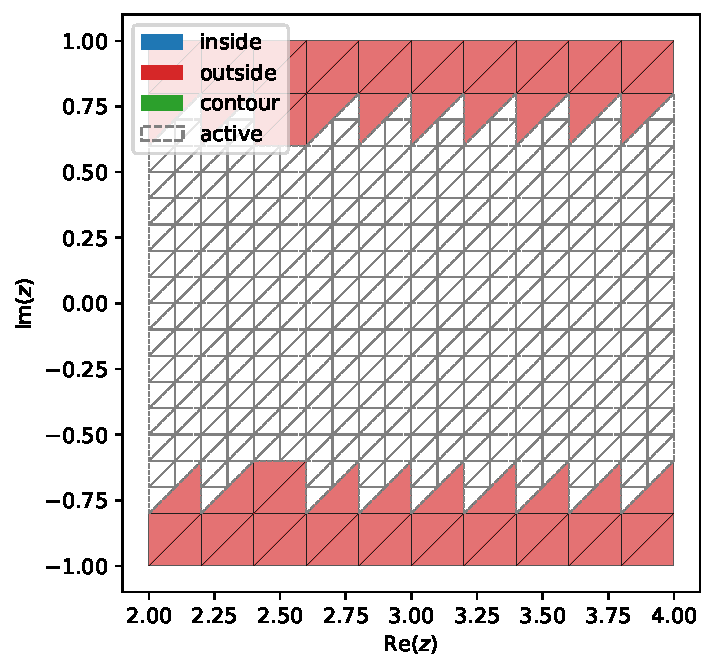
\includegraphics[width=\linewidth]{images/maxwell_sweep_000.pdf}
        \caption{Results for $\mathcal{T}_0$}
        \label{fig:sweep1}
    \end{subfigure}
    \hfill
    \begin{subfigure}[t]{0.45\textwidth}
        \centering
        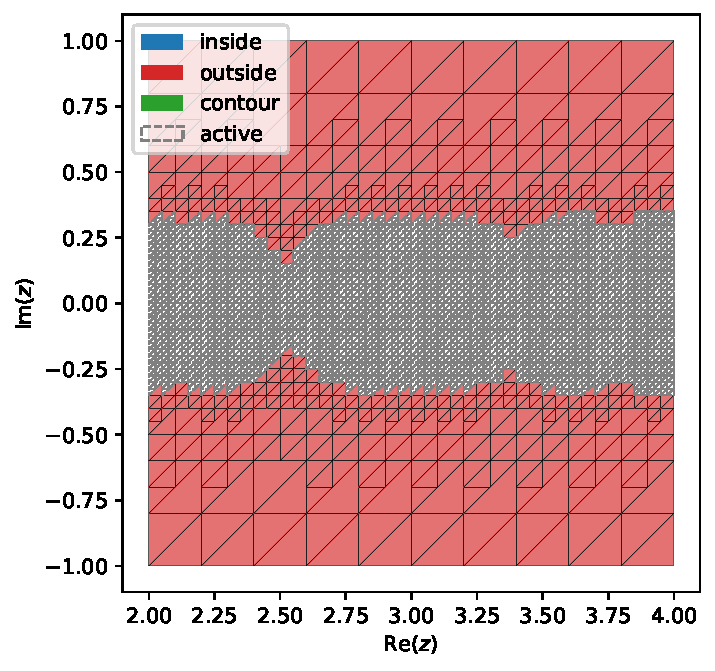
\includegraphics[width=\linewidth]{images/maxwell_sweep_002.pdf}
        \caption{Results for $\mathcal{T}_2$}
        \label{fig:sweep2}
    \end{subfigure}

    \vspace{-0.1cm}

    % Bottom row
    \begin{subfigure}[t]{0.45\textwidth}
        \centering
        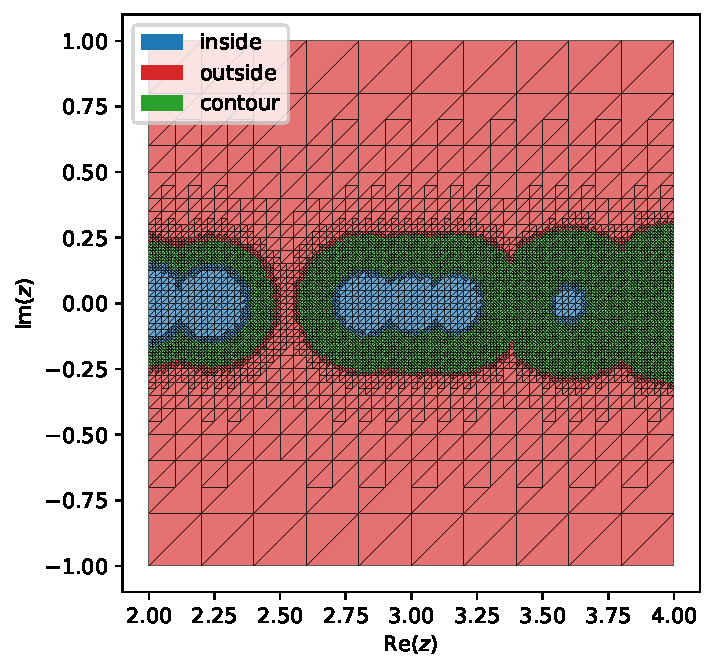
\includegraphics[width=\linewidth]{images/maxwell_sweep_004.pdf}
        \caption{Results for $\mathcal{T}_4$}
        \label{fig:sweep3}
    \end{subfigure}

    \caption[The Computed $\epsilon=0.2$ Pseudospectral Picture for the Two-Dimensional Maxwell Operator]{Selected snapshots of Algorithm \ref{outerloop} applied to the $\epsilon = 0.2$ pseudospectrum of the Maxwell operator, \eqref{max op}. The colour scheme is as in Figure \ref{dirac results}.}
    \label{maxwell sweeps}
\end{figure}